%% Преамбула TeX-файла

% 1. Стиль и язык
\documentclass[utf8x, 12pt]{G7-32} % Стиль (по умолчанию будет 14pt)
\usepackage[T2A]{fontenc}
\usepackage[russian]{babel}
\usepackage{float}
\usepackage{pdfpages}
\usepackage{tabularx}

% Остальные стандартные настройки убраны в preamble.inc.tex.
\sloppy

% Настройки стиля ГОСТ 7-32
% Для начала определяем, хотим мы или нет, чтобы рисунки и таблицы нумеровались в пределах раздела, или нам нужна сквозная нумерация.
% \EqInChapter % формулы будут нумероваться в пределах раздела
% \TableInChapter % таблицы будут нумероваться в пределах раздела
% \PicInChapter % рисунки будут нумероваться в пределах раздела

% Добавляем гипертекстовое оглавление в PDF
% \usepackage[
% bookmarks=true, colorlinks=true, unicode=true,
% urlcolor=black,linkcolor=black, anchorcolor=black,
% citecolor=black, menucolor=black, filecolor=black,
% ]{hyperref}

% Изменение начертания шрифта --- после чего выглядит таймсоподобно.
% apt-get install scalable-cyrfonts-tex

% \usepackage{cyrtimespatched}

\usepackage{setspace}

\usepackage{graphicx}   % Пакет для включения рисунков
\graphicspath{ {./images/} }

% С такими оно полями оно работает по-умолчанию:
% \RequirePackage[left=20mm,right=10mm,top=20mm,bottom=20mm,headsep=0pt]{geometry}
% Если вас тошнит от поля в 10мм --- увеличивайте до 20-ти, ну и про переплёт не забывайте:
\geometry{top=20mm}
\geometry{bottom=20mm}
\geometry{right=15mm}
\geometry{left=30mm}


% Пакет Tikz
\usepackage{tikz}
\usetikzlibrary{arrows,positioning,shadows}

% ячейки в несколько строчек
\usepackage{multirow}

% itemize внутри tabular
\usepackage{paralist,array}

% Оставить ссылки, но убрать рамки
\usepackage[hidelinks]{hyperref}

% Стили аннотаций
\usepackage{caption}
\captionsetup{font={stretch=1}}

% Times new roman
% \usepackage{mathptmx}

% Размер шрифтов для заголовков
\usepackage{titlesec}
\titleformat{\chapter}[block]{\normalfont\fontsize{14}{16}\selectfont\bfseries}{\thechapter}{1em}{}
\titleformat{\section}[block]{\fontsize{14}{16}\selectfont\bfseries}{\thesection}{1em}{}
\titleformat{\subsection}[block]{\fontsize{14}{16}\selectfont\bfseries}{\thesubsection}{1em}{}
\titleformat{\subsubsection}[block]{\fontsize{14}{16}\selectfont\bfseries}{\thesubsubsection}{1em}{}

\usepackage{tocloft}
\renewcommand{\cftbeforechapskip}{0.10cm}  % интервал между главами
\renewcommand{\cftbeforesecskip}{0.10cm}   % интервал между разделами
\renewcommand{\cftbeforesubsecskip}{0.10cm} % интервал между подразделами

% Глава (chapter) — обычный (не жирный)
\renewcommand{\cftchapfont}{\normalfont}
\renewcommand{\cftchappagefont}{\normalfont}

% Раздел (section)
\renewcommand{\cftsecfont}{\normalfont}
\renewcommand{\cftsecpagefont}{\normalfont}

% Подраздел (subsection)
\renewcommand{\cftsubsecfont}{\normalfont}
\renewcommand{\cftsubsecpagefont}{\normalfont}



\titlespacing*{\chapter}{0pt}{0pt}{0pt}
% \titlespacing*{\section}
%   {0pt}{3.5ex plus 1ex minus .2ex}{2.3ex plus .2ex}
% \titlespacing*{\subsection}{0pt}{3.5ex plus 1ex minus .2ex}{2.3ex plus .2ex}
% \titlespacing*{\subsubsection}{0pt}{3.5ex plus 1ex minus .2ex}{2.3ex plus .2ex}


% Отсупы в перечислениях
\usepackage{enumitem}
\usepackage[russian]{babel}
\AddEnumerateCounter{\asbuk}{\@asbuk}{а}
\usepackage{enumitem}
\setlist[enumerate]{
    label=\asbuk*),
    leftmargin=0.67cm, 
}

% Нумерации в библио c точками
\usepackage{etoolbox}
\makeatletter
\patchcmd{\@biblabel}{#1}{#1.}{}{}
\makeatother

% Елочка в содержании
\usepackage{tocloft}
\setlength{\cftchapindent}{0pt}      % глава без отступа
\setlength{\cftsecindent}{1em}     % отступ для \section
\setlength{\cftsubsecindent}{1.75em}    % отступ для \subsection
\setlength{\cftsubsubsecindent}{4.5em} % если используете \subsubsection

\setlength{\cftsecnumwidth}{2.5em}      % ширина для номера section
\setlength{\cftsubsecnumwidth}{3.5em}   % ширина для номера subsection
\setlength{\cftsubsubsecnumwidth}{4.5em} % ширина номера subsubsection


% Настройки листингов.
% 8 Листинги

\usepackage{listings}

% Значения по умолчанию
\lstset{
  basicstyle= \footnotesize,
  breakatwhitespace=true,% разрыв строк только на whitespacce
  breaklines=true,       % переносить длинные строки
%   captionpos=b,          % подписи снизу -- вроде не надо
  inputencoding=koi8-r,
  numbers=left,          % нумерация слева
  numberstyle=\footnotesize,
  showspaces=false,      % показывать пробелы подчеркиваниями -- идиотизм 70-х годов
  showstringspaces=false,
  showtabs=false,        % и табы тоже
  stepnumber=1,
  tabsize=4,              % кому нужны табы по 8 символов?
  frame=single
}

% Стиль для псевдокода: строчки обычно короткие, поэтому размер шрифта побольше
\lstdefinestyle{pseudocode}{
  basicstyle=\small,
  keywordstyle=\color{black}\bfseries\underbar,
  language=Pseudocode,
  numberstyle=\footnotesize,
  commentstyle=\footnotesize\it
}

% Стиль для обычного кода: маленький шрифт
\lstdefinestyle{realcode}{
  basicstyle=\scriptsize,
  numberstyle=\footnotesize
}

% Стиль для коротких кусков обычного кода: средний шрифт
\lstdefinestyle{simplecode}{
  basicstyle=\footnotesize,
  numberstyle=\footnotesize
}

% Стиль для BNF
\lstdefinestyle{grammar}{
  basicstyle=\footnotesize,
  numberstyle=\footnotesize,
  stringstyle=\bfseries\ttfamily,
  language=BNF
}

% Определим свой язык для написания псевдокодов на основе Python
\lstdefinelanguage[]{Pseudocode}[]{Python}{
  morekeywords={each,empty,wait,do},% ключевые слова добавлять сюда
  morecomment=[s]{\{}{\}},% комменты {а-ля Pascal} смотрятся нагляднее
  literate=% а сюда добавлять операторы, которые хотите отображать как мат. символы
    {->}{\ensuremath{$\rightarrow$}~}2%
    {<-}{\ensuremath{$\leftarrow$}~}2%
    {:=}{\ensuremath{$\leftarrow$}~}2%
    {<--}{\ensuremath{$\Longleftarrow$}~}2%
}[keywords,comments]

% Свой язык для задания грамматик в BNF
\lstdefinelanguage[]{BNF}[]{}{
  morekeywords={},
  morecomment=[s]{@}{@},
  morestring=[b]",%
  literate=%
    {->}{\ensuremath{$\rightarrow$}~}2%
    {*}{\ensuremath{$^*$}~}2%
    {+}{\ensuremath{$^+$}~}2%
    {|}{\ensuremath{$|$}~}2%
}[keywords,comments,strings]

% Подписи к листингам на русском языке.
\renewcommand\lstlistingname{\cyr\CYRL\cyri\cyrs\cyrt\cyri\cyrn\cyrg}
\renewcommand\lstlistlistingname{\cyr\CYRL\cyri\cyrs\cyrt\cyri\cyrn\cyrg\cyri}


% Полезные макросы листингов.
% Любимые команды
\newcommand{\Code}[1]{\textbf{#1}}
\newcommand{\eqspace}[0]{\setlength\abovedisplayskip{3.2ex}\setlength\belowdisplayskip{3.2ex}\setlength\abovedisplayshortskip{3.2ex}\setlength\belowdisplayshortskip{3.2ex}}

\begin{document}

\frontmatter % выключает нумерацию ВСЕГО; здесь начинаются ненумерованные главы: реферат, введение, глоссарий, сокращения и прочее.

% Команды \breakingbeforechapters и \nonbreakingbeforechapters
% управляют разрывом страницы перед главами.
% По-умолчанию страница разрывается.

% \nobreakingbeforechapters
\breakingbeforechapters

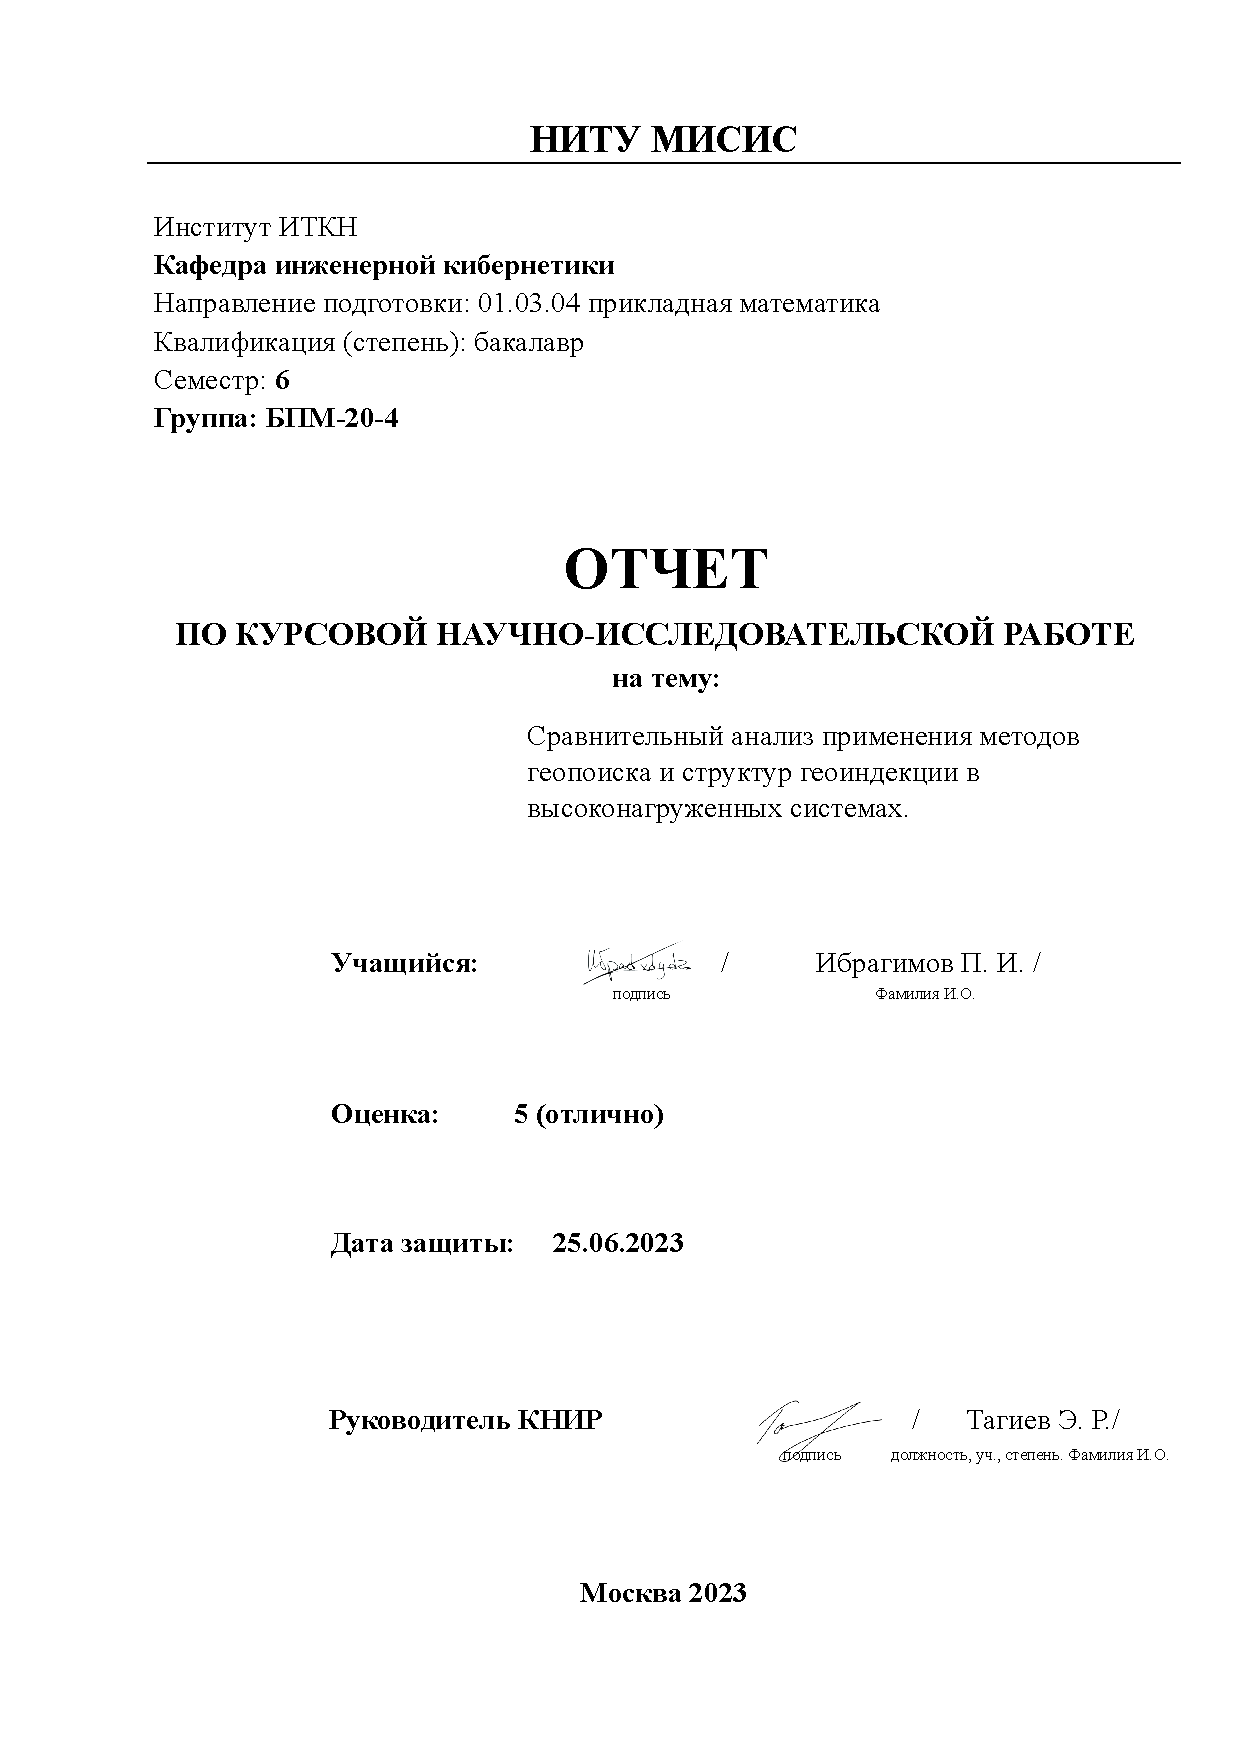
\includepdf{pdf/title-page.pdf}

%%% Local Variables:
%%% mode: latex
%%% TeX-master: "rpz"
%%% Stop:


\tableofcontents

  \Defines % Необходимые определения. Вряд ли понадобться
\begin{description}
    \item[Индекс] Абстрактная структура данных упрощающая операции поиска
    \item[Геоиндекс] Индекс, построенный для упрощения поиска по геоданным
\end{description}

%%% Local Variables:
%%% mode: latex
%%% TeX-master: "rpz"
%%% Stop:

\Abbreviations %% Список обозначений и сокращений в тексте
В настоящей КНИР применяют следующие сокращения и обозначения:

\noindent СУБД --- Система управления базами данных

\noindent БД --- База данных

\noindent SQL (Structured Query Language) --- Язык структурированных запросов. Декларативный язык запросов для взаимодействия с СУБД. Используется в таких базах данных как: Postgres, MySQL, MSSQL, SQLite и тд.

\noindent RPS (Requests per second) --- Запросов за секунду. Метрика оценки нагруженности системы по количество запросов от клиентов серверу в секундах.

\noindent KNN (k-nearest neighbors) - К-ближайщих соседей, задача поиска К-ближайших соседей к точке А по метрике D.

%%% Local Variables:
%%% mode: latex
%%% TeX-master: "rpz"
%%% Stop:

\Introduction

В настоящее время геоданные являются неотъемлемой частью многих высоко нагруженных систем, таких как поисковые системы, социальные сети, картографические сервисы и другие. Однако обработка и хранение большого объема геоданных может стать проблемой для разработчиков. Для решения данной проблемы были разработаны методы геопоиска и пространственные индексы, которые позволяют эффективно работать с геоданными в высоко нагруженных системах.

Цель данной дипломной работы — провести сравнительный анализ применения алгоритмов геопоиска и пространственных индексов в высоко нагруженных системах. В работе будут рассмотрены основные принципы работы данных методов, их преимущества и недостатки. Также будет проведено сравнение производительности данных методов на различных наборах геоданных.

Под высоконагруженной системой подразумевается система, в которой нет возможности бесконечно масштабировать систему вертикально и разработчикам приходится оптимизировать существующие алгоритмы и подходы. Часто, такая система имеет большое количество запросов как на чтение, так и на запись, а общее количество запросов к системе в секунду (RPS) превышает несколько тысяч. 

Основной проблемой работы с геоданными в высоко нагруженных системах является неочевидность в выборе структур и методов хранения данных. Так, например, классический индекс B-Tree нельзя использовать при обращении к кортежам геоточек, потому что B-Tree умеет работать только со скалярными данными. При этом для работы с геоданным существует объемное количество индексов, например, R-Tree, KD-Tree, Quadtree, каждый из которых имеет свои плюсы и минусы. Помимо этого существует проблема сериализации и десериализации данных, которая заключается в том, что результаты анализа поиска, запросы на поиск и сами данных точек необходимо передавать по сети в как можно меньшем объеме и размере (в данном случае под объемом подразумевается количество передаваем данных, а размер — вес в байтах).

Результаты данной работы могут быть полезны для разработчиков высоко нагруженных систем, которые работают с геоданными, а также для специалистов в области геоинформатики.



\chapter{АНАЛИТИЧЕСКИЙ ОБЗОР ЛИТЕРАТУРЫ}
\label{cha:analysis}

В данной работе будут анализироваться только 2 задачи поиска по геоданным. Задачи можно сформулировать следующим образом:
Пусть есть множество точек, представляющих собой пару широта-долгота, отображающих некий объект на поверхности земли.

Надо:
\begin{enumerate}
    \item Найти все объекты Х, находящиеся на растояние У от объекта Z. Эту задачу можно переформулировать следующим образом: найти все объекты множества Х в окружности c радиусом Y и центром в Z.
    \item Найти X ближайщих объектов к объекту Z. Эта задача также известна как задача поиска ближайших соседей.
\end{enumerate}

\subsection{Расстояние между двумя точками}
Указанные выше задачи требуют обусловить понятие расстояния между двумя геоточками. Для этого введем понятие геоточки: это точка, представляющая собой кортеж A(x, y), где x и y - широта и долгота соответственно.
Расстоянием между двумя точками есть наименьшая примая на плоскости земного шара, при этом ее вычисление может быть разным в зависиомости от положеной задачи. \\
Поставим задачу:

Даны геоточки $A(x_1, y_1), B(x_2, y_2)$. Требуется найти растояние $d(A, B)$

\subsubsection{Евклидово расстояние}
В некоторых системах, например, расширение Postgis для СУБД Postgres для типа Geometry, используется евклидово расстоние:

$$
d(A, B)=\sqrt{(x_1-x_2)^2+(y_1-y_2)^2}
$$

Данный подход работает корректно только в части случаев, так, например, он выдаст правильный результат с точностью до 5 метров в случае поиска растояния в пределах Москвы, но, расстояние в Африке будет отличаться в 2-3 раза относительно более корректных подходов.
При это важно отметить, что данная дистанция отвечает аксиомам метрики, поэтому ее корректно использовать при сравнение расстояний между двумя точками, например, при решение задаче KNN(К-ближайших соседей).

\subsubsection{Расстояние гаверсинуса}
Расстояние гаверсинуса - это способ определения расстояния между двумя точками на поверхности Земли, учитывающий кривизну Земли. Оно используется в геопоиске для определения расстояния между заданной точкой и объектами в заданном радиусе.

Формула расстояния гаверсинуса выглядит следующим образом:

$$
d(A, B) = 2R \cdot \arcsin\left(\sqrt{\sin^2\left(\frac{x_2-x_1}{2}\right) + \cos(x_1) \cdot \cos(x_2) \cdot \sin^2\left(\frac{y_2-y_1}{2}\right)}\right)
$$

где d - расстояние между двумя точками в километрах, R - радиус Земли (приблизительно 6371 км), $x_1$ и $x_2$ - широты двух точек в радианах, $y_1$ и $y_2$ - долготы двух точек в радианах.

Эта формула позволяет определить расстояние между точками с точностью до нескольких метров, что делает ее очень полезной для геопоиска. Однако, она может быть достаточно ресурсоемкой при работе с большими объемами геоданных, что делает ее медленее по сравнению с Евклидовым расстоянием.

\subsubsection{Геодезическое расстояние}
Геодезическое расстояние - это расстояние между двумя точками на поверхности Земли, измеренное вдоль кратчайшей линии (геодезической линии) между этими точками. Геодезическая линия - это кривая на поверхности Земли, которая имеет наименьшую длину между двумя точками.

Геодезическое расстояние учитывает кривизну Земли и может отличаться от расстояния гаверсинуса, особенно на больших расстояниях и при использовании разных моделей формы Земли.

Для расчета геодезического расстояния используются различные методы, такие как метод Винсента, метод Гаусса-Крюгера и метод Хаверсина. Эти методы учитывают форму Земли и позволяют получить более точные результаты, чем простые формулы для расчета расстояния на плоскости.

Геодезическое расстояние широко используется в геопозиционировании, навигации, картографии и других областях, где требуется точное определение расстояния между двумя точками на поверхности Земли.

Формула вычисления геодезии:
$$
d(A, B) = R \cdot \arccos(\sin(x_1) \cdot \sin(x_1) + \cos(x_1) \cdot \cos(x_2) \cdot \cos(y_2 - y_1)
$$


\subsection{Структуры геоиндексации}
Как и с задачами поиска по \textit{плоскому} массиву скаляров, для поиска по геокординатам используются специальные структуры данных, которые позволяют оптимизировать операции поиска. \\
Указанные структуры можно разбить на 2 типа: древовидные и плоские. К первому виду относятся: R-tree, R*-tree, Quad-tree, K-d tree. К плоским относятся: Geohash, S2 и H3. \\
Расмотрим принцип работы древовидных структур на примере K-d tree.\\
\subsubsection{K-d tree}
K-d tree представляет собой дерево, позволяющее производить операции поиска в N-мерном пространстве. Расмотрим двухмерное K-d tree, которое также можно назвать K-2 tree.
Само K-D tree является обычным бинарным сбалонсированным деревом.
Алгоритм построенния K-d tree довольно прост:
\begin{enumerate}
    \item Происходит поиск центральной точки, то есть той точки, которая будет находится на сумарно меньшем растояние от всех точек. Данная точка ставиться в корень дерева k-d tree.
    \item Далее плоскость "разбивается" на 2 части по вертикальной оси
    \item "Слева" ищется "средняя точка", то есть та точка, которая по оси абсцис(широте) находится на сумарно меньшем расстояние до остальных. Данная точка записывает в левого ребенка корня дерева
    \item Аналогичная процедура повторяется справа.
    \item Аналогичная процедура повторяется для вновь созданых полотен, но уже с осью ординат(долготой)
    \item Данные процедуры повторяются со всеми точками.
\end{enumerate}
\subsection{Процесс поиска по K-d tree}
Процесс поиска K ближайших точек и всех точек в заданном радиусе очень поход на процесс поиска по бинарному дереву за тем исключением, что при сравнение по четным нодам идет по широте, а по нечетным - по долготе.

\subsubsection{Geohash}
Geohash(далее также геохеш), в отличие от древовидных структур преставляет собой обычный массив, поиск по которому можно реализовывать через тривиальные методы, например, через бинарное дерево поиска, красно-черные деревья или b-tree.
Самим геохешом называется строка, закодированная 32 разрядным алфавитом, перевод из 10-ой системы в указанный алфавит указан в таблице ниже.
\begin{center}
\begin{tabular}{ c|c c c c c c c c }
 Основание 10 & 0 & 1 & 2 & 3 & 4 & 5 & 6 & 7 \\
 Основание 32 & 0 & 1 & 2 & 3 & 4 & 5 & 6 & 7 \\
  \hline\hline
 Основание 10 & 8 & 9 & 10 & 11 & 12 & 13 & 14 & 15 \\
 Основание 32 & 8 & 9 & b & c & d & e & f & g \\
  \hline\hline
 Основание 10 & 16 & 17 & 18 & 19 & 20 & 21 & 22 & 23  \\
 Основание 32 & h & j & k & m & n & p & q & r \\
  \hline\hline
 Основание 10 & 24 & 25 & 26 & 27 & 28 & 29 & 30 & 31 \\
 Основание 32 & s & t & u & v & w & x & y & z \\
\end{tabular}
\end{center}
Данная строка однозначно декодируется в кортеж геокоординат с некой точностью, зависящей от количества символов в строке. Примеры:
\begin{enumerate}
    \item строка \texttt{ucft} дегодируется в прямоугольник площадью примерно 800 $ km^2 $ и центром в (55.81, 37.44).
    \item строка \texttt{ucft943} имеет тот же центр - (55.8236, 37.3116), но меньшую площадь $23409 m^2$
\end{enumerate}
Как можно наблюдать, чем выше количество символов, используемых в геохеше, чем выше точность получаемых координат, но при этом выше затрачиваемая память.
В данной работе не будет детально описываться процесс формарования геохеша за исключением базового принципа: \\
Сфера земли разбивается на практически равные прямоугольники, после чего каждому прямоугольнику присваивается номер в 32х ричной системе координат, номера присваиваются в порядке "змейкой", сначала самый левый-верхний, далее ниже от него, далее справа от самого левого-верхнего и тд. \\

\subsection{Сравнительный анализ}
Чтобы дать корректный ответ на вопрос о том, какую струтуру данных стоит использовать, введем следующие критерии сравнения:
- занимаемый объем памяти
- время предподготовки данных
- время поиска K ближайщих соседей
- время поиска по радиусу и точке
- время вставки точки
- время удаления точки

При этом для чистоты эксперемента стоит добавить следующие ограничения:
- Не будет учитываться время записи на диск. Предпологается, что все операции производятся при использование оперативной памяти.
- Требуется учитывать как теоретические показатели, то есть O-нотацию, так и практические результаты.


%%% Local Variables:
%%% mode: latex
%%% TeX-master: "rpz"
%%% End:


\Conclusion

В ходе исследования был проведен сравнительный анализ применения методов геопоиска и структур геоиндекции в высоконагруженных системах. Было выявлено, что все стркутуры имеют свои преимущества и недостатки, и выбор между ними зависит от конкретных задач и требований к системе.

Древесные методы R-tree, KD-tree позволяют быстро находить объекты на карте, но требует больших вычислительных ресурсов при обработке больших объемов данных. Geohash, Uber H3, S2 Geometry, в свою очередь, позволяют эффективно хранить и обрабатывать большие объемы геоданных, но могут быть менее точными в поиске объектов.

Таким образом, выбор между методами геопоиска должен основываться на конкретных требованиях к системе и ее возможностях. Важно учитывать как скорость поиска объектов, так и эффективность использования ресурсов системы.

При этом важно отметить, что в высоконагруженных системах данные методы могут комбинироваться для достижения наилучших результатов, например, использовать Geohash для поиска в местах, где не требуется точность, а R-tree для аналитики данных через холодные хранилищах.

В работе удалось полностью достичь поставленных целей.

В следующем семестре будет решаться более прикладная проблема, а именно сравнительный анализ конкретных реализаций структур с целью выявления узких мест в реализациях. Потребуется реализовать все приведенные структуры и провести нагрузочное тестирование, чтобы можно было найти все крайние случаи работы указанных подходов. Для решения данной задачи будут применятся научная дисциплина Информатика, для реализации структур и проведения нагрузочного тестирования будет использоваться язык Golang.

За время выполнения работы мною было познано знание относительно формирования геохешей, а также устройство работы многомерных деревьей: R-tree, KD-tree и тд.

% % Список литературы при помощи BibTeX
% Юзать так:
%
% pdflatex rpz
% bibtex rpz
% pdflatex rpz

\bibliographystyle{gost2800}
\bibliography{rpz}

\begin{enumerate}
    \item A. Guttman. R-trees: A Dynamic Index Structure for Spatial Searching. Proceedings of ACM SIGMOD, pages 47-57, 1984
    \item N. Beckmann, H.P. Kriegel, R. Schneider and B. Seeger. The R*-tree: An Efficient and Robust Access Method for Points and Rectangles. Proceedings of ACM SIGMOD, pages 323-331, May 1990.
    \item N. Roussopoulos, S. Kelley and F. Vincent. Nearest Neighbor Queries. ACM SIGMOD, pages 71-79, 1995.
    \item Sahr, Kevin (2019). Central Place Indexing: Hierarchical Linear Indexing Systems for Mixed-Aperture Hexagonal Discrete Global Grid Systems. Cartographica: The International Journal for Geographic Information and Geovisualization, 54(1), 16–29. doi:10.3138/cart.54.1.2018-0022
    \item  Jiajun Liu, Haoran Li, Yong Gao, Hao Yu, Dan Jiang. [IEEE 2014 22nd International Conference on Geoinformatics - Kaohsiung, Taiwan (2014.6.25-2014.6.27)] 2014 22nd International Conference on Geoinformatics - A geohash-based index for spatial data management in distributed memory. 2014

\end{enumerate}

%%% Local Variables:
%%% mode: latex
%%% TeX-master: "rpz"
%%% Stop:


\end{document}

%%% Local Variables:
%%% mode: latex
%%% TeX-master: t
%%% End:
